% !TEX encoding = UTF-8
% !TEX TS-program = pdflatex
% !TEX root = ../tesi.tex
% !TEX spellcheck = it-IT

%*************************************************************
\chapter{Implementazione del sistema}
\label{cap:implementazione}
%*************************************************************

Questo capitolo descrive la fase dello sviluppo del sistema, partendo dall'architettura presentata nel paragrafo \ref{par:architettura-del-sistema}, per poi scendere nel dettaglio dei vari componenti.

\section{Sviluppo componenti del sistema}
Coerentemente con l'architettura illustrata in figura \ref{fig:architettura-sistema} si è implementato ogni componente del sistema. Per lo sviluppo dei vari componenti si sono utilizzati dei framework. In figura \ref{fig:color-coded} si riporta il grafico color coded dei vari componenti del sistema dove in azzurro sono evidenziate le parti sviluppate mentre in verde sono indicati i framework e i moduli utilizzati. Di seguito si descrive, in ordine di sviluppo, l’implementazione di ogni componente del sistema.

\begin{figure}[htp]
	\centering
	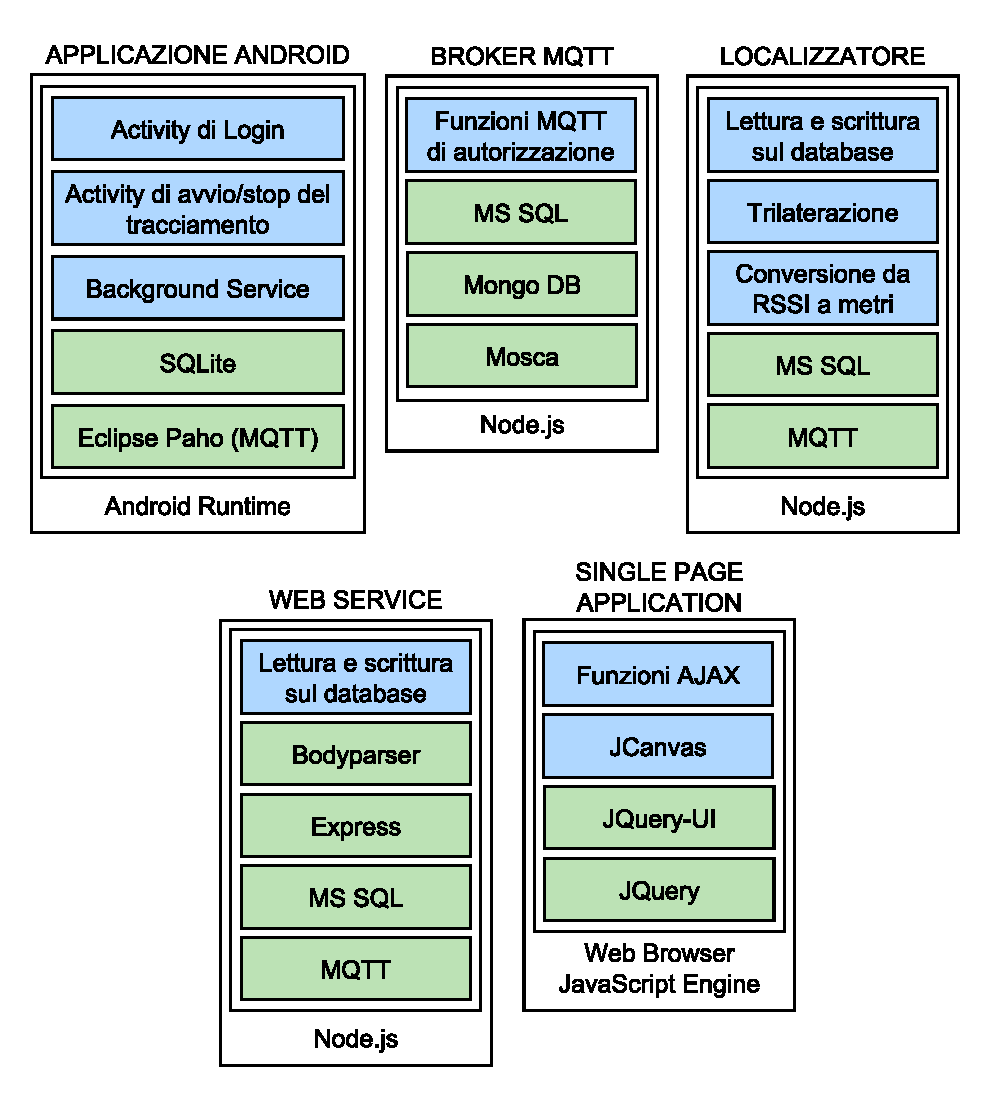
\includegraphics[height=10 cm]{color-coded}
	\caption{Grafico color coded dei componenti sviluppati}
	\label{fig:color-coded}
\end{figure}

\section{Database}
Il motore del database centrale è Microsoft SQL Server, coerentemente con quanto imposto nei vincoli di progetto. Per l’immagazzinamento dei dati si è realizzato il modello entità-relazione rappresentato in figura \ref{fig:modello-er-db-centrale}. Il database contiene quattro entità in relazione tra loro. Le entità sono:
\begin{description}
	
	\item[UTENTE] si occupa di memorizzare i dati relativi ad un utente che può accedere al sistema;
	
	\item[TRACCIA] si occupa di memorizzare le tracce dei vari utenti;
	
	\item[POSIZIONE] contiene per ogni traccia le coordinate dell'ambiente indoor;
	
	\item[TAG BLE] contiente le informazioni riguardanti la posizione di ogni TAG BLE.
	
\end{description}
Le relazioni che intercorrono tra le entità sono:
\begin{description}
	
	\item[Registra] per ogni utente possono essere presenti una o più tracce con datetime diverso per ogni traccia.
	
	\item[Corrisponde] ad ogni traccia applicando l'algoritmo di trilaterazione corrsiponde una sola posizione e viceversa;
	
	\item[Contiene] ogni traccia contiene 3 TAG BLE i quali possono avere valori di RSSI diversi ed ogni TAG BLE può essere presente in più tracce;
	
\end{description}
Utilizzando il modello ER appena presentato si è costruito il modello relazionale e, infine, si è applicata la procedura di normalizzazione per minimizzare la ridondanza dei dati.

\begin{figure}[htp]
	\centering
	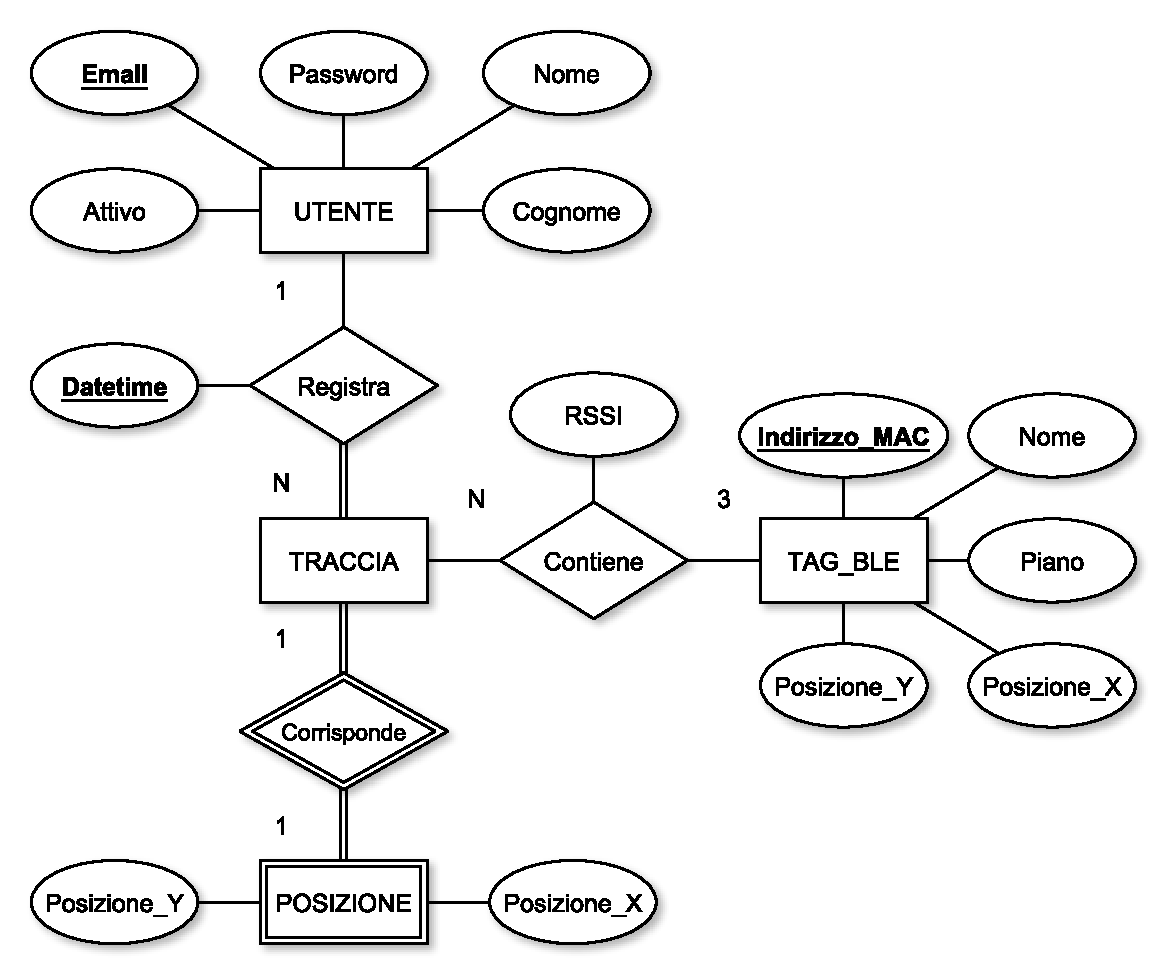
\includegraphics[height=\textheight/3]{modello-er-db-centrale}
	\caption{Modello E-R del database centrale}
	\label{fig:modello-er-db-centrale}
\end{figure}

\section{Broker MQTT}
Per lo sviluppo del broker MQTT si è scelto di utilizzare il broker Mosca. Mosca \cite{mosca:site} è un broker MQTT che può essere integrato in applicazioni Node.js. Il broker implementa diverse caratteristiche, tra cui: MQTT 3.1 e 3.1.1, QoS 0 e QoS 1, varie opzioni di archiviazione per i pacchetti offline QoS 1 e le sottoscrizioni. Per avere la garanzia nella comunicazione, si deve utilizzare un database. Mosca offre la compatibilità con diversi database non relazionali. Si è scelto di utilizzare il database MongoDB che si occuperà di rendere disponibili le funzioni di:
\begin{description}
	
	\item[Keep-Alive message] il broker riesce a identificare una disconnessione non esplicita del client;
	
	\item[Will message] viene impostato nel messaggio di CONNECT con topic, QoS e retain. In caso di disconnessione inaspettata il messaggio ``Will'' viene mandato ai subscribers registrati;
	
	\item[Retain message] un messaggio pubblicato su un topic viene mantenuto sul broker. Un successivo subscriber che si connette sullo stesso topic riceve il messaggio (last known good message).
	
	\item[Persistent Session] dopo la disconnessione del client, tutte le sottoscrizioni vengono mantenute nel broker e recuperate alla connessione successiva.
	
\end{description}
Dopo aver integrato il broker seguendo le linee guida della documentazione, si sono riscritte le funzioni che permettono di verificare se un utente può utilizzare o meno il sistema. La funzione di autenticazione, visibile nel listato \ref{cod:auth-broker}, utilizza la libreria Mssql per interfacciarsi con Microsoft SQL Server.
\begin{lstlisting}[language=JavaScript, label=cod:auth-broker, caption=Funzione di autenticazione del broker MQTT]
// Autenticazione
authenticate = function(client, email, password, callback) {
var autorizzato = false;
return mssql.connect(sqlConfig).then(function() {
var request = new mssql.Request(mssql);
// conta gli utenti che hanno la stessa email e password
var stringRq = "SELECT COUNT(*) AS presente FROM utente WHERE Email = '" + email + "' AND Password = '" + password + "';";
// autorizzo se presente altrimenti rifiuto la connessione
return request.query(stringRq).then(function(result) {
autorizzato = result[0].presente == 1;
if (!autorizzato) { // email non autorizzata
	return callback(null, autorizzato); }
else { // email autorizzata
	client.user = email;
	return callback(null, autorizzato); }
mssql.close(); })
.catch(function (err) {
console.log(err);
mssql.close(); });
}).catch(function (err) {
console.log(err); });
}
\end{lstlisting}

\section{Localizzatore}
Il localizzatore è un componente che si occupa di interfacciarsi con il database utilizzando il protocollo MQTT. Si è utilizzata la libreria MQTT.js che implementa le funzioni del protocollo MQTT per Node.js. Il localizzatore, al suo avvio, deve pubblicare la lista di tutti i TAG BLE presenti nel database centrale con il flag retain.
Quando il broker riceve da un utente un messaggio contenente un insieme di tracce, il broker lo inoltra al localizzatore. Il localizzatore a questo punto, memorizza le tracce ricevute nel database e successivamente effettua prima la conversione da RSSI a metri, poi ottenendo la posizione relativa dei TAG BLE interessati effettua il calcolo della posizione eseguendo l'algoritmo di Trilaterazione.

\subsection{Conversione da RSSI a metri}
La conversione da RSSI a metri si è implementata nel localizzatore con il codice visibile nel listato \ref{cod:rssi-to-meter}, coerentemente con quanto spiegato nel paragrafo \ref{par:ranging}. 

\begin{lstlisting}[language=JavaScript, label=cod:rssi-to-meter, caption=Conversione da RSSI a Metri]
// Conversione da RSSI a Metri
calcoloRssiMetri = function(rssi) {
	var A = -40 // potenza del segnale ricevuto in campo aperto
	var n = 2 // costante di propagazione in campo aperto
	
	var esponente = (A - rssi) / (10 * n);
	return Math.pow(10,esponente);
}
\end{lstlisting}

\subsection{Algoritmo di Trilaterazione}
L'algoritmo di Trilaterazione si è implementato seguendo quanto indicato nel paragrafo \ref{par:trilaterazione}. In primo luogo si implementa una funzione che permetta di calcolare il punto medio di un array di punti. La firma della funzione è visibile nel listato \ref{cod:media-punti}.

\begin{lstlisting}[language=JavaScript, label=cod:media-punti, caption=Calcolo del punto medio]
getMediaPunti = function(punti) { /* ... */ }
\end{lstlisting}

Successivamente si definisce una funzione che ritorna il punto medio della Trilaterazione iterata per tutti e tre i nodi beacon, visibile nel listato \ref{cod:esegui-trilaterazione}.

\begin{lstlisting}[language=JavaScript, label=cod:esegui-trilaterazione, caption=Calcolo del punto medio della Trilaterazione iterata per i tre nodi beacon]
trilaterazione = function(x1, y1, d1, x2, y2, d2, x3, y3, d3) {
	return getMediaPunti(new Array(
	getTrilaterazione(x1, y1, d1, x2, y2, d2, x3, y3, d3),
	getTrilaterazione(x3, y3, d3, x1, y1, d1, x2, y2, d2),
	getTrilaterazione(x2, y2, d2, x3, y3, d3, x1, y1, d1)))
}
\end{lstlisting}


Infine si scrive l'algoritmo di Trilaterazione, visibile nel listato \ref{cod:trilaterazione}, risolvendo il sistema di equazioni \ref{eq:sistema-trilaterazione}.


\begin{lstlisting}[language=JavaScript, label=cod:trilaterazione, caption=Algoritmo di trilaterazione]
getTrilaterazione = function(x1, y1, d1, x2, y2, d2, x3, y3, d3) {
var r = new Object(); // è l'oggetto da ritornare
// verifico se i due cerchi si incrociano
if (Math.sqrt(Math.pow(x1-x2,2) + Math.pow(y1-y2,2)) <= (d1+d2)) {
var a1=-2*x1; var b1=-2*y1; var a2=-2*x2; var b2=-2*y2;
var c1=Math.pow(x1,2)+Math.pow(y1,2)-Math.pow(d1,2);
var c2=Math.pow(x2,2)+Math.pow(y2,2)-Math.pow(d2,2);
if(a1 != a2) { // ricavo le coordinate del polinomio
var a=1+Math.pow(b2-b1,2)/Math.pow(a1-a2,2);
var b=2*(b2-b1)*(c2-c1)/Math.pow(a1-a2,2)+(a1*(b2-b1))/(a1-a2)+b1;
var c=Math.trunc(c1+a1*(c2-c1)/(a1-a2)+Math.pow(c2-c1,2)/Math.pow(a1-a2,2));
// risolvo l'eq. di secondo grado a*x^2 + b*x + c
var delta = Math.sqrt(Math.pow(b,2) - 4*a*c);
var ys1=(-b+delta)/(2*a); var ys2=(-b-delta)/(2*a);
// ricavo i due valori di x risolvendo l'eq.
var xs1=(c2-c1)/(a1-a2)+((b2-b1)*ys1)/(a1-a2);
var xs2=(c2-c1)/(a1-a2)+((b2-b1)*ys2)/(a1-a2);
// se le due soluzioni sono uguali ho il punto di intersezione
if(xs1==xs2 && ys1==ys2) { r.x=xs1; r.y=ys1; return r; }
else { // altrimenti la distanza del nodo stimato dal terzo anchor
d1=Math.sqrt(Math.pow(xs1-x3,2)+Math.pow(ys1-y3,2));
d2=Math.sqrt(Math.pow(xs2-x3,2)+Math.pow(ys2-y3,2));
if ((d1-d3)<(d2-d3)) { r.x=xs1; r.y=ys1; return r; }
else { r.x=xs2; r.y=ys2; return r;}
}}
else { // ricavo le coordinate del polinomio
var a=1+Math.pow(a2-a1,2)/Math.pow(b1-b2,2);
var b=2*(a2-a1)*(c2-c1)/Math.pow(b1-b2,2)+(b1*(a2-a1))/(b1-b2)+a1;
var c=Math.trunc(c1+b1*(c2-c1)/(b1-b2)+Math.pow(c2-c1,2)/Math.pow(b1-b2,2));
// risolvo l'eq. di secondo grado a*x^2 + b*x + c
var delta=Math.sqrt(Math.pow(b,2)-4*a*c);
var xs1=(-b+delta)/(2*a); var xs2=(-b-delta)/(2*a);
// ricavo i due valori di y risolvendo l'eq.
var ys1=(c2-c1)/(b1-b2)+((a2-a1)*xs1)/(b1-b2);
var ys2=(c2-c1)/(b1-b2)+((a2-a1)*xs2)/(b1-b2);
// se le due soluzioni sono uguali ho il punto di intersezione
if(xs1==xs2 && ys1==ys2) { r.x=xs1; r.y= ys1; return r; }
else { // altrimenti la distanza del nodo stimato dal terzo anchor
d1=Math.sqrt(Math.pow(xs1-x3,2)+Math.pow(ys1-y3,2));
d2=Math.sqrt(Math.pow(xs2-x3,2)+Math.pow(ys2-y3,2));
if ((d1-d3)<(d2-d3)) { r.x=xs1;	r.y=ys1; return r; }
else { r.x = xs2; r.y = ys2; return r;}
}}}
else { // altrimenti se i due cerchi non si incrociano
var dr=(Math.sqrt(Math.pow(x1-x2,2)+Math.pow(y1-y2,2))-(d1+d2))/2;
// nuovi raggi
d1 += dr;	d2 += dr;
return getTrilaterazione(x1, y1, d1, x2, y2, d2, x3, y3, d3);
}}
\end{lstlisting}

\section{Web Service}
Il web service si occupa di rendere disponibili le varie funzioni per la Single Page Application. Per lo sviluppo si sono utilizzate le seguenti librerie:
\begin{description}
	
	\item[MQTT.js] per pubblicare al broker MQTT la lista dei TAG BLE, se questi vengono modificati dalla SIngle Page Application, con il flag retain;
	
	\item[Express] per realizzare le varie funzioni REST del webservice;
	
	\item[Body-parser] per effettuare il parsing middleware del corpo del messaggio ricevuto dalla Single Page Application;
	
	\item[Mssql] per interfacciarsi con Microsoft SQL Server.
	
\end{description}
Si sono sviluppate le varie API del web service utilizzando prevalentemente le librerie Express e Mssql, effettuando delle interrogazioni SQL specifiche per poi inviare alla Single Page Application i dati richiesti.


\section{Single Page Application}
La Single Page Application offre all'utente la possibilità di configurare i TAG BLE e di vedere le risorse all'interno dell'ambiente indoor desiderato.
I casi d'uso implementati sono visibili in figura \ref{fig:ucs-spa}.
Per lo sviluppo dell'applicazione si sono utilizzati i seguenti framework:
\begin{description}
	
	\item[JQuery] utilizzato per le chiamate AJAX e per il supporto multibrowser;
	
	\item[JQuery-UI] utilizzato per creare le varie maschere di inserimento e modifica dei dati riguardanti alla configurazione dei TAG BLE;
	
	\item[JCanvas] utilizzato per disegnare sulla mappa dell’ambiente indoor e per animare i movimenti real time delle varie risorse monitorate.
	
\end{description}
Si è utilizzato, inoltre, a corredo dei framework JavaScript sopra citati anche il linguaggio HTML e CSS per definire la struttura e l’aspetto grafico dell'applicazione.

\begin{figure}[htp]
	\centering
	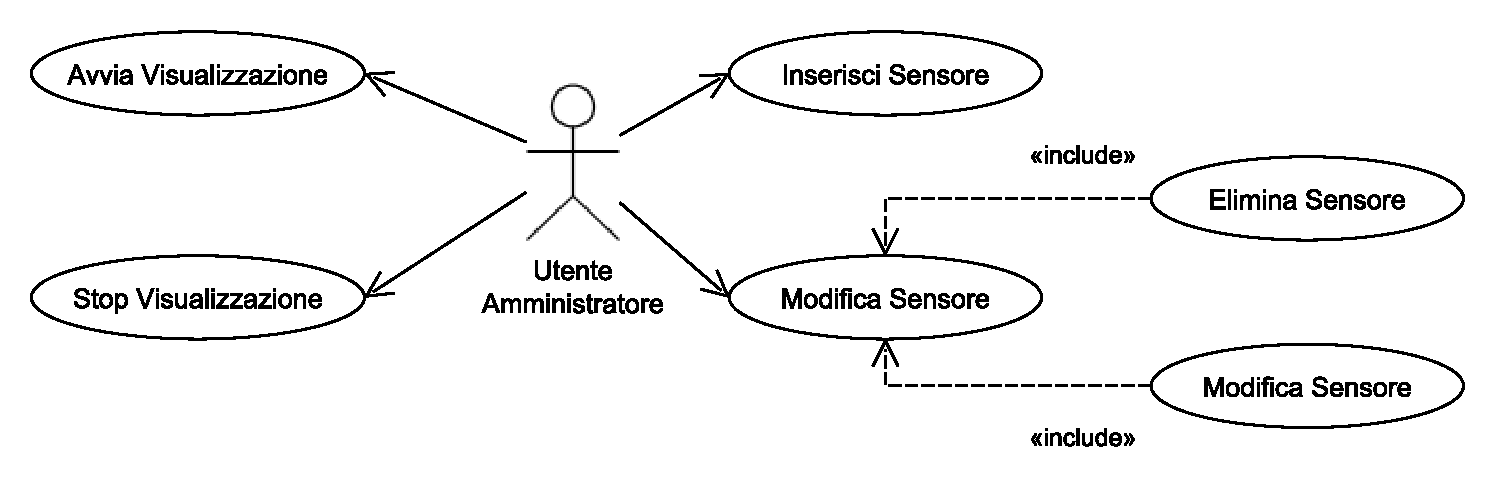
\includegraphics[width=\textwidth]{ucs-spa}
	\caption{Casi d'uso Single Page Application}
	\label{fig:ucs-spa}
\end{figure}

\section{Applicazione Android}
L'applicazione Android contiene due activity: l'activity di login e l'activity per avviare o fermare la rilevazione della risorsa. L’activity di login si interfaccia con l’utente chiedendo di inserire email e password per verificare la possibilità di accedere al sistema. L'activity di gestione della rilevazione si avvia automaticamente una volta che l'autenticazione è andata a buon fine. Le due activity e i casi d'uso ad esse associate, sono visibili in figura \ref{fig:ucs-android}.
Per la gestione dei dati si utilizza il database SQLite presente sul sistema operativo Android. Si realizza, quindi, il diagramma entità-relazione, rappresentato in figura \ref{fig:modello-er-db-android}.

\begin{figure}[htp]
	\centering
	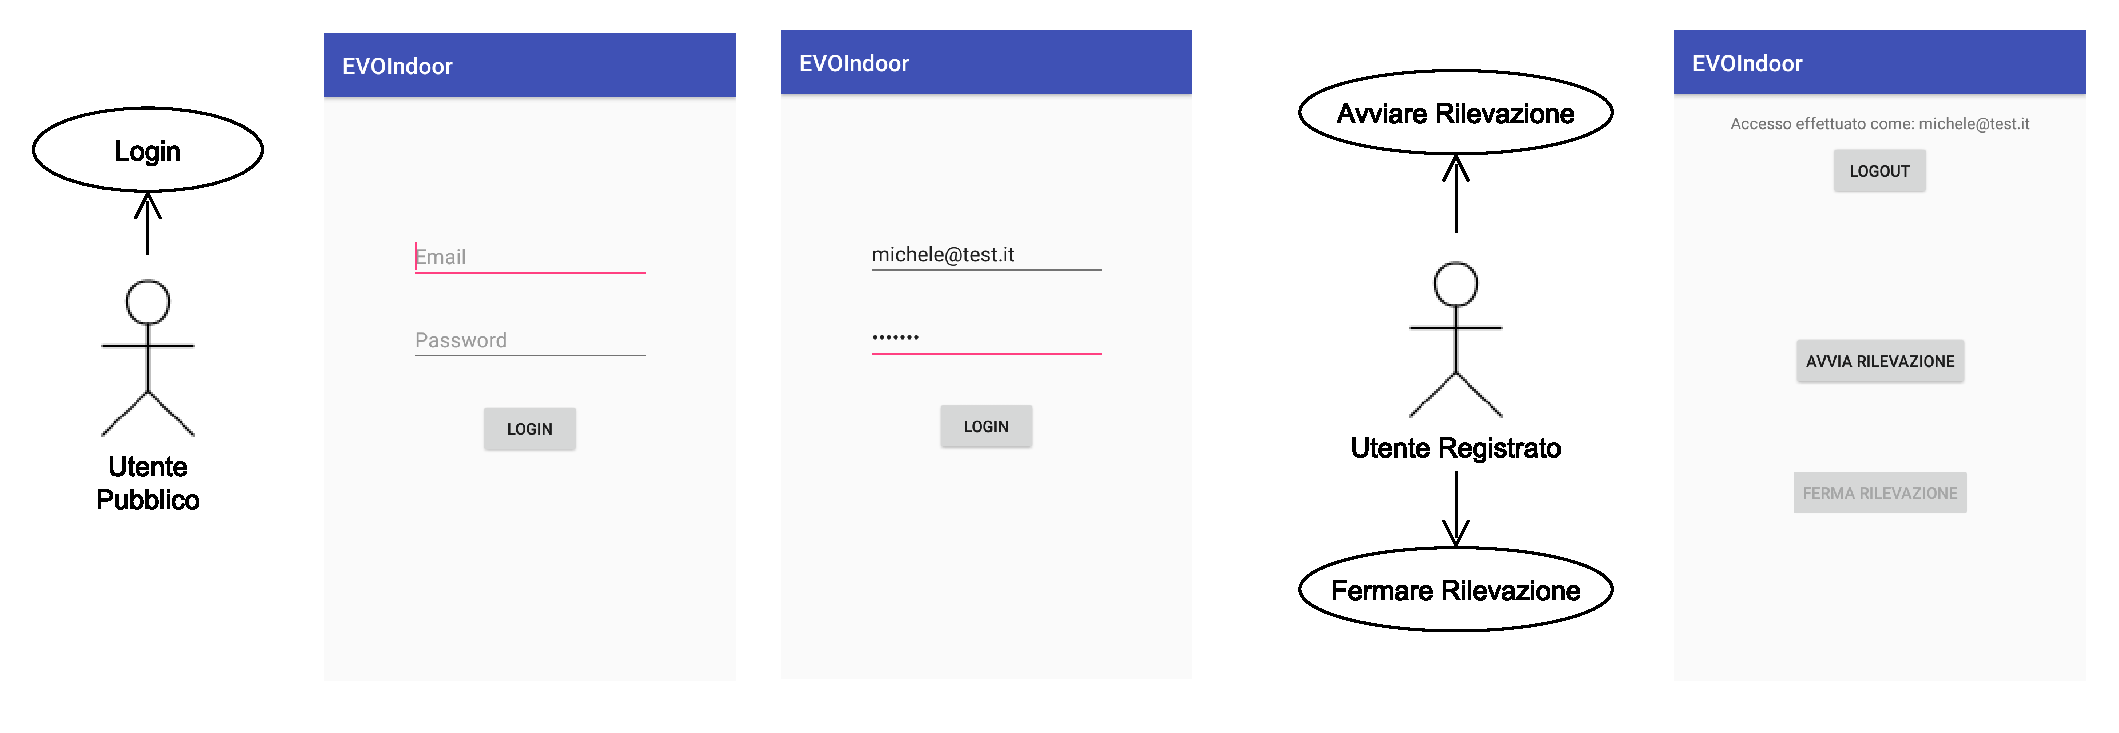
\includegraphics[width=\textwidth]{ucs-android}
	\caption{Casi d'uso applicazione Android}
	\label{fig:ucs-android}
\end{figure}

\begin{figure}[htp]
	\centering
	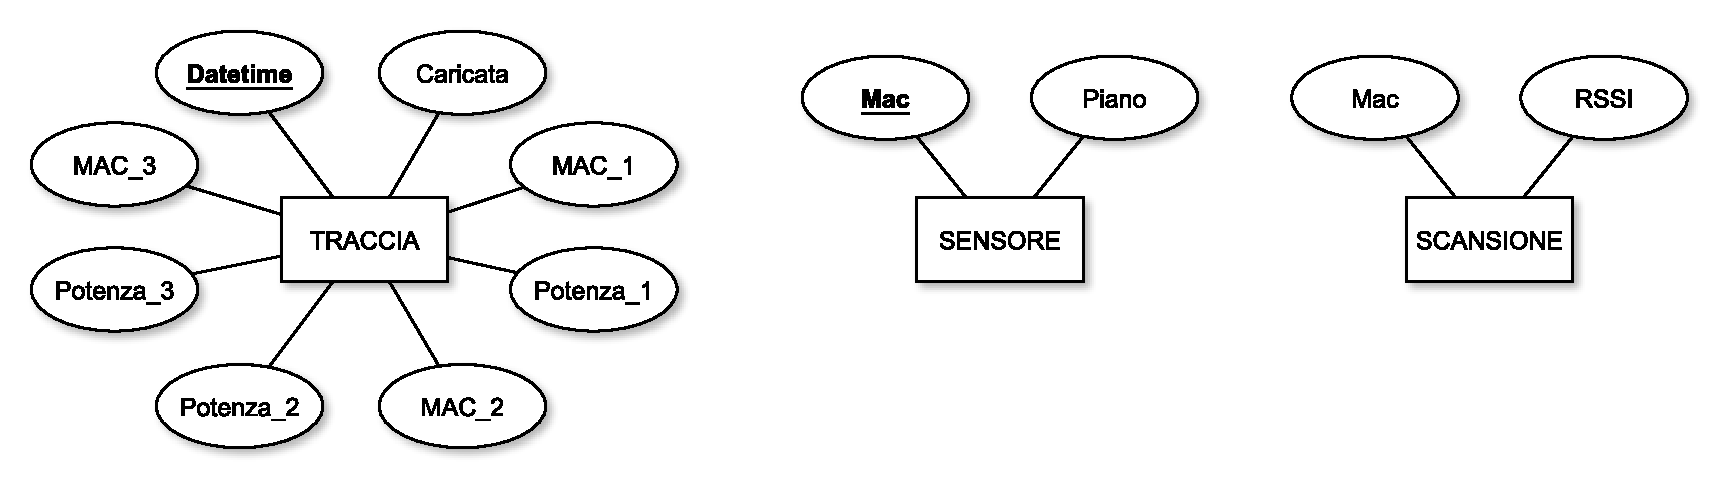
\includegraphics[width=\textwidth]{modello-er-db-android}
	\caption{Modello E-R del database dell'applicazione Android}
	\label{fig:modello-er-db-android}
\end{figure}

Per lo sviluppo delle funzioni del protocollo MQTT si è utilizzata la libreria Eclipse Paho, libreria di riferimento per l’ecosistema MQTT, disponibile open-source in diversi linguaggi.
Al suo avvio la seconda Activity effettua la sottoscrizione al topic in cui è presente la lista dei TAG BLE e, dato che o il localizzatore o il web service hanno pubblicato sullo stesso topic la lista dei TAG BLE disponibili con flag retain, allora si riceve subito la lista dei TAG BLE.

La lista dei TAG BLE serve per poter filtrare durante la scansione dei dispositivi Bluetooth solo quelli che effettivamente risultano essere registrati nella piattaforma, evitando in questo modo di memorizzare l'RSSI di altre periferiche che implementano l’interfaccia Bluetooth LE.

All'avvio della rilevazione, si avvia un service in background composto da due thread \texttt{TracciaUpload} e \texttt{TracciaBuffer}.

Il thread \texttt{TracciaBuffer} finchè la rilevazione è attiva esegue sequenzialmente le seguenti operazioni:
\begin{enumerate}
	
	\item Avvia la scansione dei dispositivi BLE;
	
	\item Attende un secondo;
	
	\item Ferma la scansione dei dispositivi BLE;
	
	\item Filtra le letture dei dispositivi BLE memorizzati, eliminando le letture dei dispositivi che non sono presenti nella lista dei TAG BLE;
	
	\item Esegue la media se sono presenti più valori di RSSI riferiti allo stesso TAG BLE;
	
	\item Aggiunge la traccia al Database, se esistono le letture di almeno 3 TAG BLE distinti, inserendo all'interno della traccia le letture dei 3 TAG BLE con indice RSSI più basso.
	 
\end{enumerate}
La scansione dei dispositivi BLE è realizzata mediante il codice \ref{cod:ble-scan}.

\begin{lstlisting}[language=JavaScript, label=cod:ble-scan, caption=Scansione dei dispositivi BLE]
BluetoothAdapter.startLeScan:
	Callback{
		db.addScansione();
	}
\end{lstlisting}

Il thread \texttt{TracciaUpload} avvia il thread \texttt{TracciaBuffer} e finchè la rilevazione è attiva esegue sequenzialmente le seguenti operazioni:
\begin{enumerate}
	
	\item Attende 2 secondi;
	
	\item Apre una connessione MQTT verso il broker;
	
	\item Invia le tracce memorizzate nel database non ancora inviate;
	
	\item Cancella le tracce inviate dal database;
	
	\item Chiude la connessione MQTT.
	 
\end{enumerate}